\chapter{Opis użytych algorytmów}
Projekt został wyposażony w trzy algorytmy wyszukujące słów podobnych pod względem budowy dla bazowego ciągu znaków, który nie występuje w użytym słowniku. 

\section{Odległość Levenshteina}
Pierwszym z użytych algorytmów jest algorytm na obliczanie długości Levenshteina (edycyjnej). Odległość ta jest miarą odmienności napisów. W algorytmie tym wyróżnia się takie pojęcie jak działanie proste na napisie. Do działań takich zaliczamy:
\begin{itemize}
	\item wstawienie nowego znaku do napisu;
	\item usunięcie znaku z napisu;
	\item zamianę znaku w napisie na inny znak;
\end{itemize}

Algorytm ten posłużył w projekcie do przeszukiwania %TODO: dokonczyc

\begin{figure} [H]
	\centering
	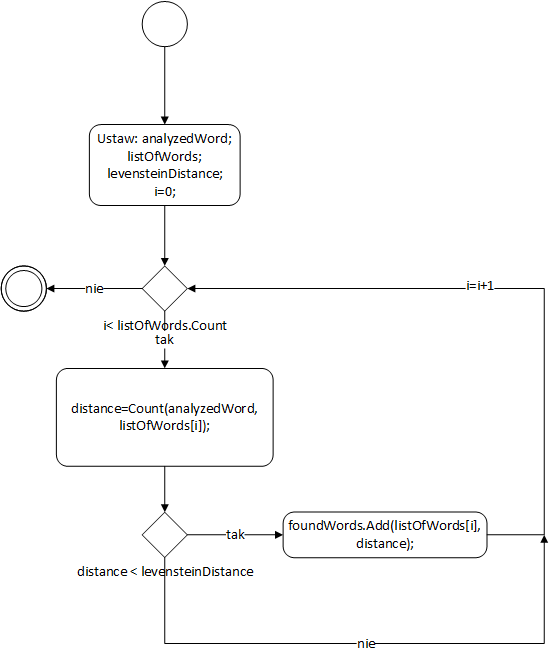
\includegraphics[width=0.6\linewidth]{rozdzial02/Levenstein1.png}
	\caption{Diagram dla działania algorytmu z wykorzystaniem odległości Levensteina}
	\label{fig:Lev}
\end{figure}

\begin{figure} [H]
	\centering
	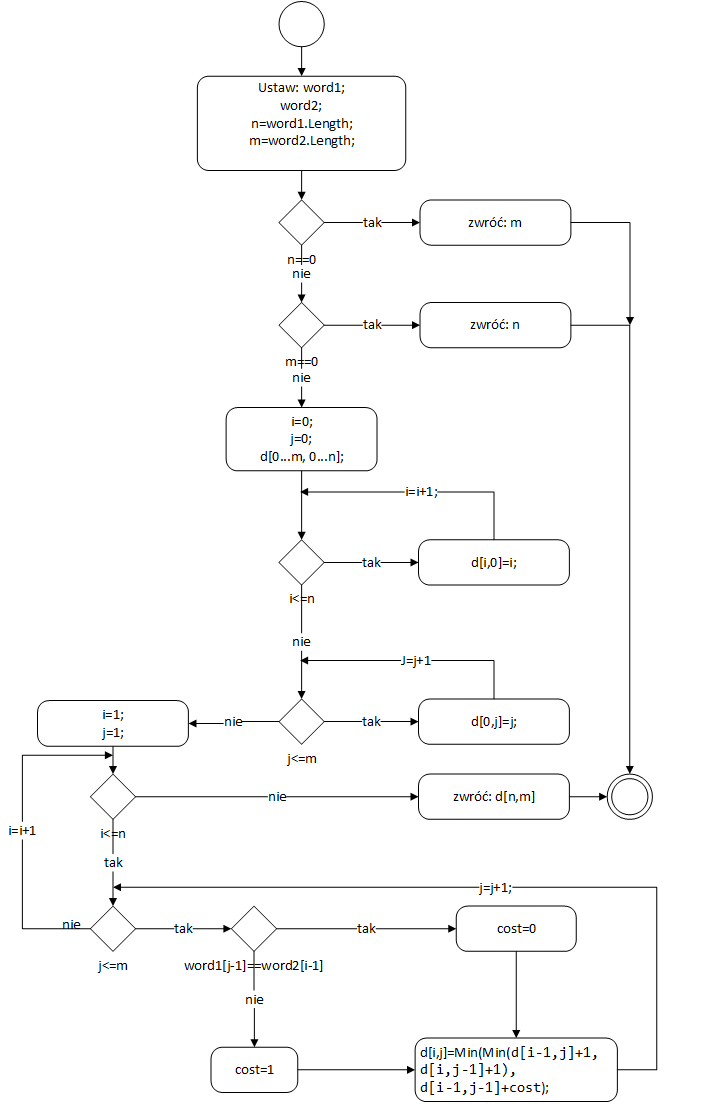
\includegraphics[width=1\linewidth]{rozdzial02/Levenstein-Count.png}
	\caption{Diagram obliczania odległości Levensteina}
	\label{fig:Lev-Count}
\end{figure}


\section{LetterChanger}

\lssetdef
\lstinputlisting[captionpos=b,caption={Lista par ciągów znakowych odpowiadająca najczęstszym błędom w języku polskim},label={lst:letter},basicstyle={\footnotesize\ttfamily}]{rozdzial02/letterPairs.txt}

\begin{figure} [H]
	\centering
	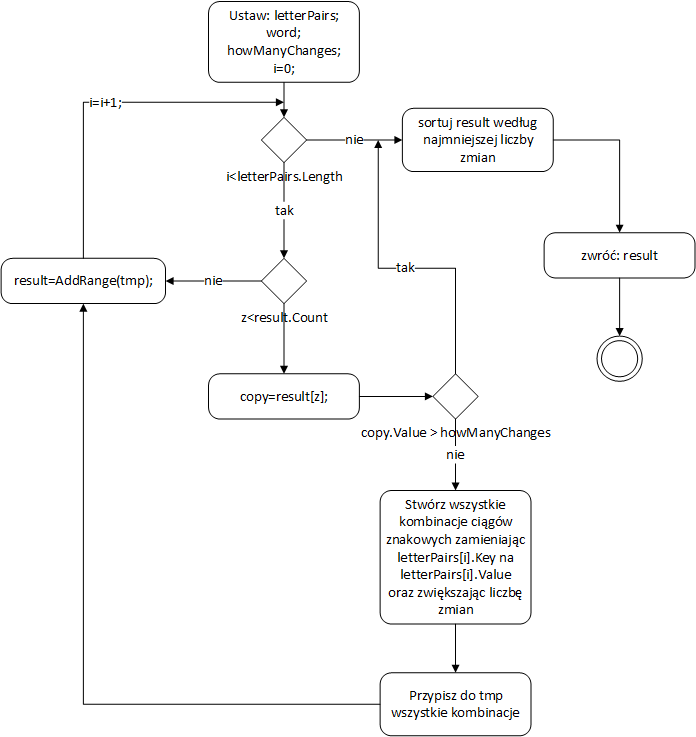
\includegraphics[width=1\linewidth]{rozdzial02/LetterChanger.png}
	\caption{Diagram zamieniania ciągów znaków odpowiadających najczęstszym błędom ortograficznym}
	\label{fig:LetterChanger}
\end{figure}

\section{SpaceAdder}

\begin{figure} [H]
	\centering
	
\includegraphics[width=0.6\linewidth]{rozdzial02/SpaceSearcher.png}
	\caption{Diagram działania funkcji dodającej przerwy między wyrazami}
	\label{fig:SpaceAdder}
\end{figure}



